\chapter{User Interface}


\subsection{Search for a Charge Point}
\begin{figure}[h]
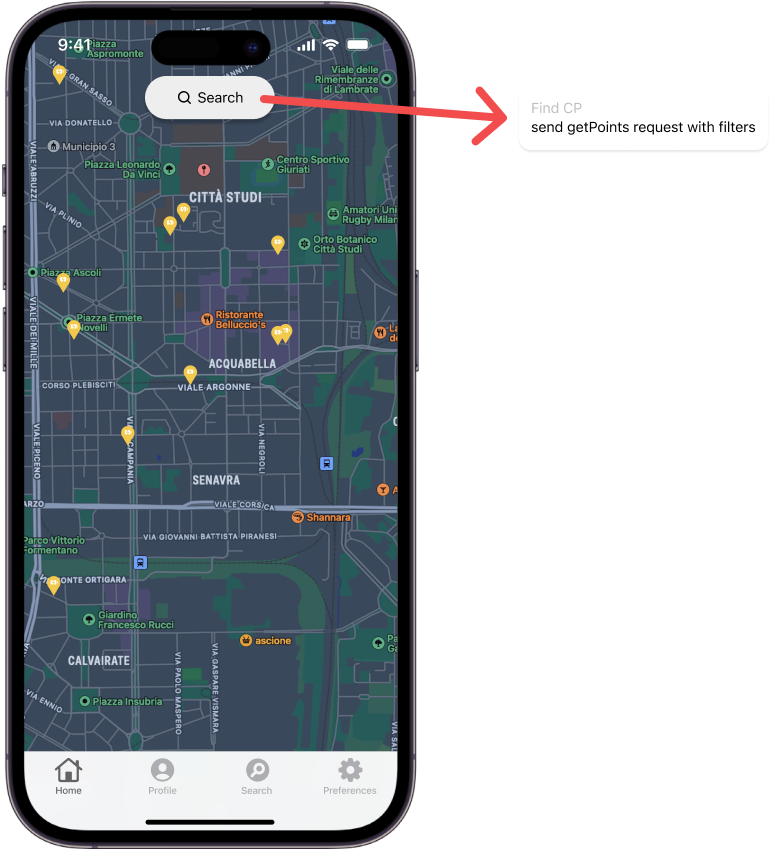
\includegraphics[width=10cm]{UI/search}
\caption{Search for a Charge Point}
\end{figure}
In this first view, the user has the ability to view all the CP nearby via the map. The datapoints are loaded via an API request to the Geo Service that returns all the points. The user can also search for a specific CP using both the "Search" button on the upper part of the map, as also using the tab button on the bottom of the application.


\subsection{Details of a CP and booking of a session}
\begin{figure}[h]
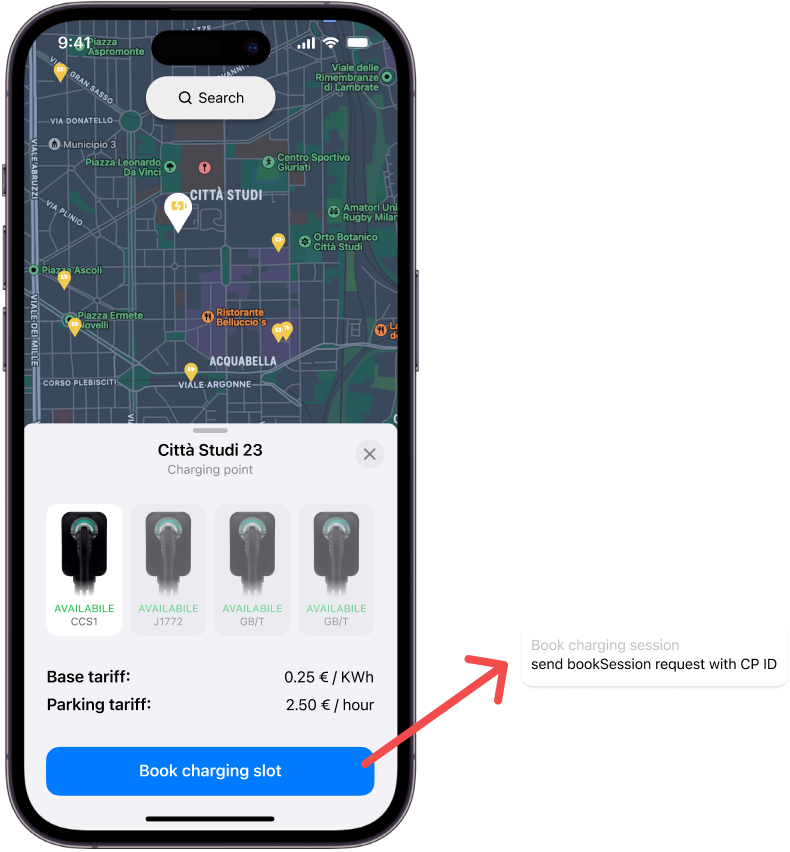
\includegraphics[width=10cm]{UI/booking}
\caption{Details of a CP and booking of a session}
\end{figure}
After tapping on a CP icon on the map, the user will be presented with the details of the selected CP, with all the plugs available and the tariffs.
Then, the user can decide to book the charging slot by selecting the connector type that he needs and by tapping onto the "Book charging slot" button. 
A bookSession request is forwarded to the Booking Service, than the OCPI Service is used to send the correct request to the selected CPMS.
After some time the CPMS will push the session to the eMSP system and the Notification Service will send a push notification to the user and will update the UI
\clearpage


\subsection{Starting the charging process}
\begin{figure}[h]
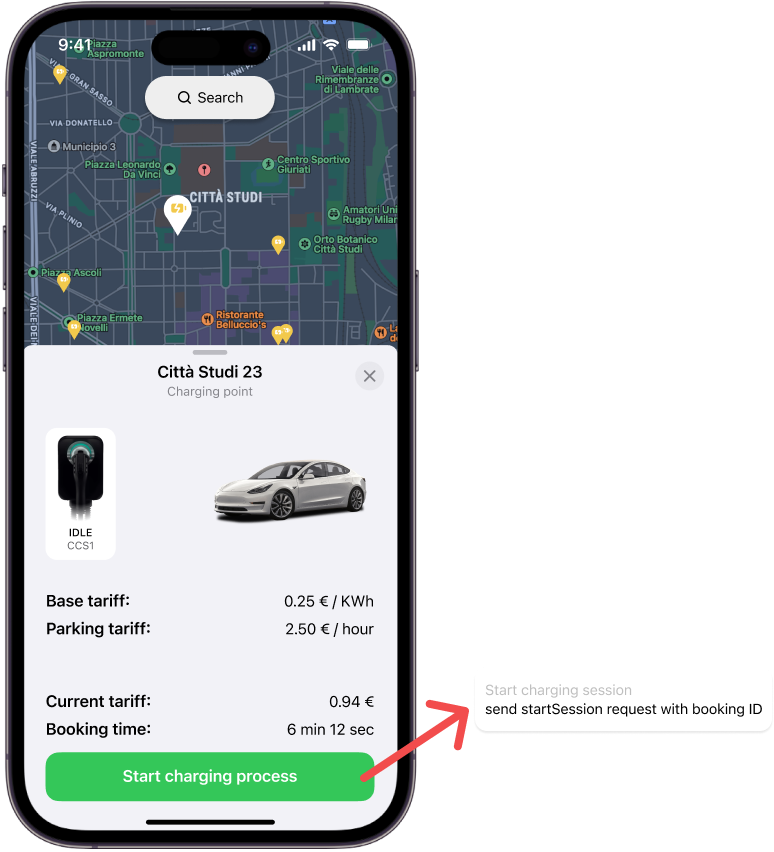
\includegraphics[width=10cm]{UI/start}
\caption{Starting the charging process}
\end{figure}
After the update received by the CPMS, a session will start and the booking details will be updated to show the current tariff that will be applied and the booking time already passed. The user, once he's reached the CP and has connected the EV to the station, can start the charging process via the "Start charging process" button. The startSession request will be sent to the Booking Service that will forward the request to the CPMS by using the OCPI Service. As the previous request, the CPMP will push the update on the booking session.
\clearpage

\subsection{Completing the charging process}
\begin{figure}[h]
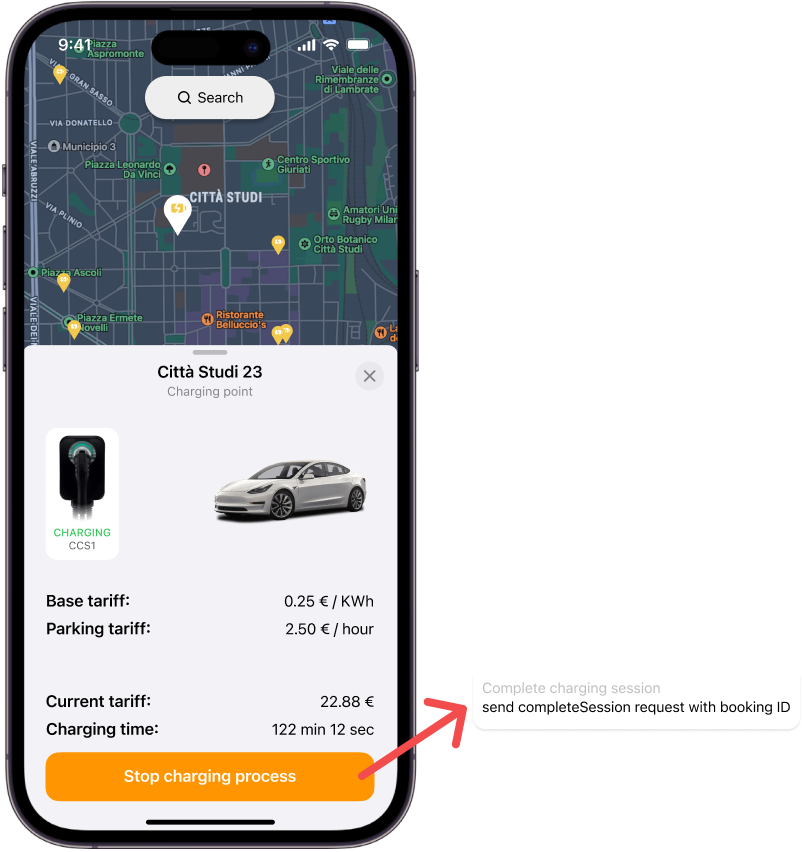
\includegraphics[width=10cm]{UI/complete}
\caption{Completing the charging process}
\end{figure}

At any time the user can view the status of the booking, updated with the latest info pushed by the CPMS. He can also complete the charging process by tapping the "Stop charging process" button. A completeSession request will be forwarded via the Booking Service to the OCPI Service that will send the correct command to the CPMS. After the confirmation from the CPMS, the user will be charged automatically via the PSP Service with the complete tariff communicated by the CPMS.
\clearpage

\subsection{Push notification from Charging Point}
\begin{figure}[h]
\centering
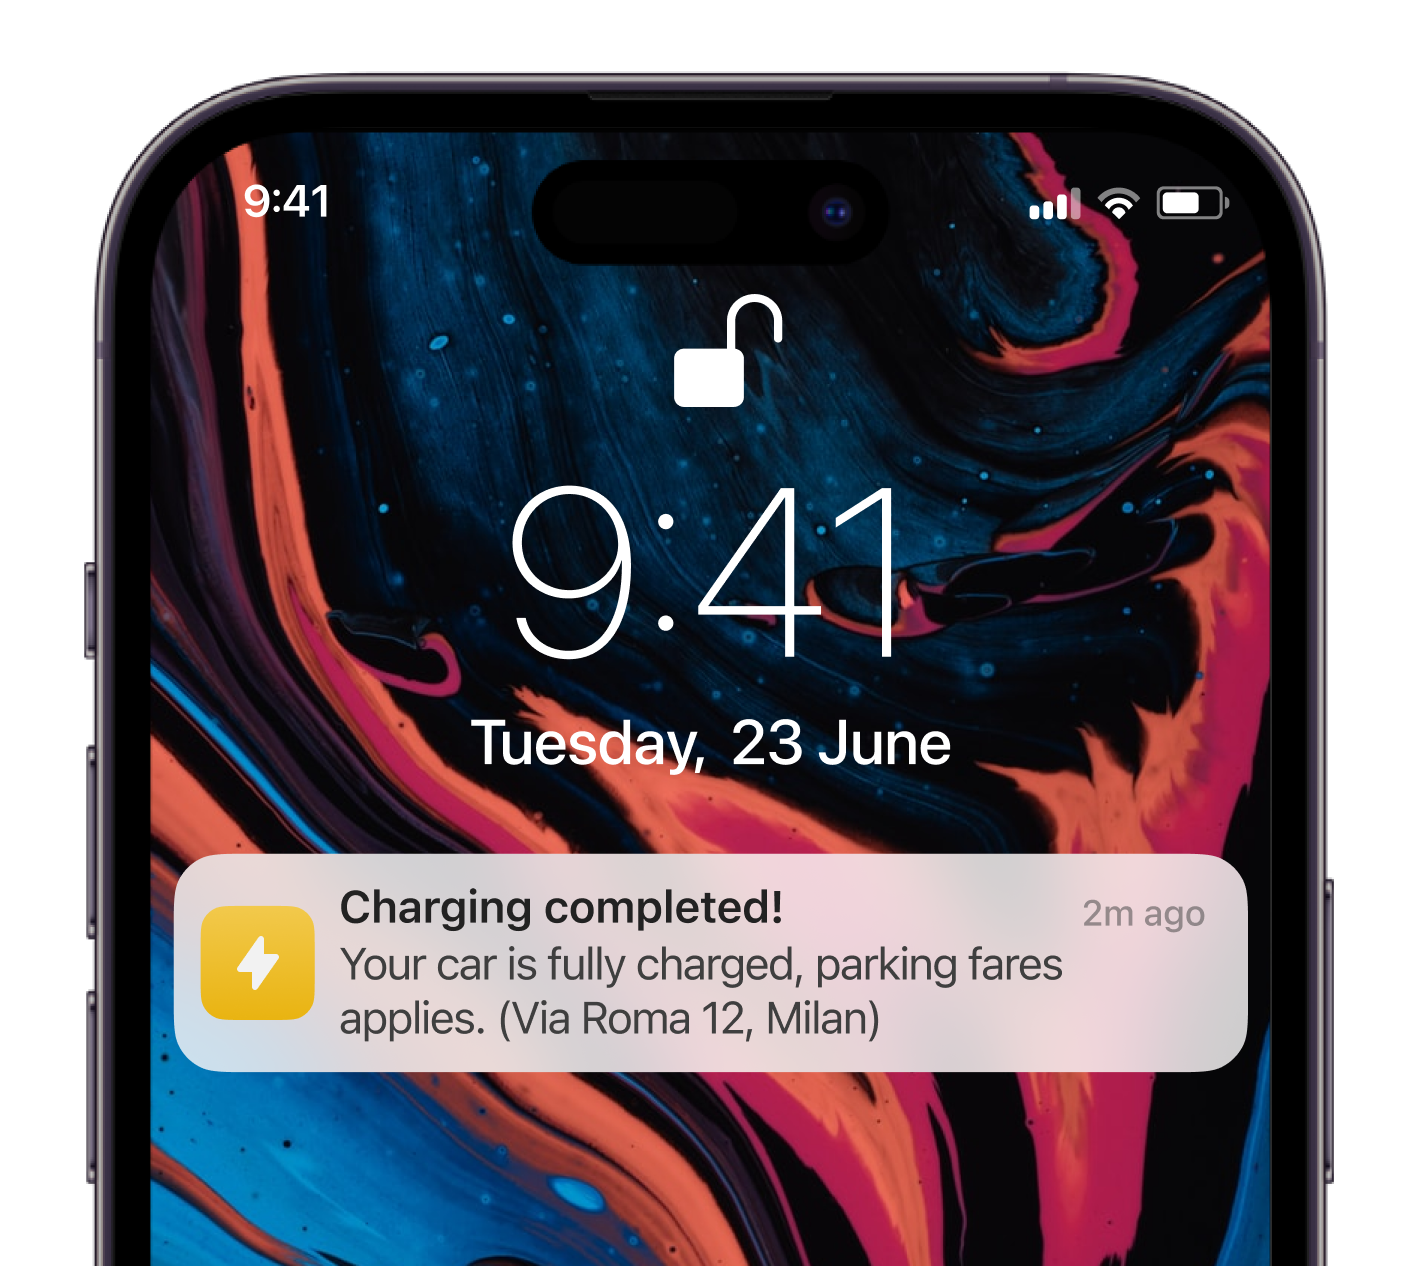
\includegraphics[width=10cm]{UI/notification}
\caption{Push notification from Charging Point when the charging session has been completed}
\end{figure}

When the CPMS push an update to the system to notify the end of the charging process, the System will send a push notification to the user, reminding them that the parking fares might be applied.









